\chapter{PROCEDURES}
\thumbtab{Procedures}{0}
\localtableofcontents
\cleardoublepage

\marginfigeometry

\section{START-UP}

\subsection{PRE-START}
\begin{checklistenumerate}
    \blueitem{\hyperref[fig:proc:prestart:flcscheck]{FLCS Check}}{
    \marginpar{
        \captionsetup{type=figure}
        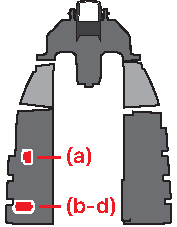
\includegraphics[width=\marginparwidth]{F16_proc_start-up_flcs-check_v01.pdf}
        \caption{\textbf{FLCS Check}}
        \label{fig:proc:prestart:flcscheck}
    }
    \begin{subenumerate}
        \item \textbf{Main PWR Switch}\cbstart \dotfill \textbf{BATT}\cbend
        \begin{itemize}
            \item \textbf{FLCS RLY Light} --- \textbf{ON}
        \end{itemize}
        \item \textbf{FLCS PWR TEST} \dotfill \textbf{TEST (hold)}
        \item \textbf{Test Lights} \dotfill \textbf{Verify}
        \begin{itemize}
            \item \textbf{ACFT BATT TO FLCS} --- \textbf{ON}
            \item \textbf{FLCS PMG} --- \textbf{ON}
            \item \textbf{FLCS PWR} --- \textbf{ON}
            \item \textbf{FLCS RLY} --- \textbf{OFF}
        \end{itemize}
        \item \textbf{FLCS PWR TEST} \dotfill \textbf{Release}
    \end{subenumerate}}
    \blueitem{\hyperref[fig:proc:prestart:mainpower]{Main Power}}{
    \marginpar{
        \captionsetup{type=figure}
        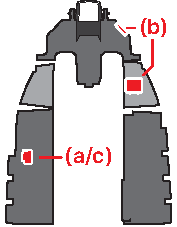
\includegraphics[width=\marginparwidth]{F16_proc_start-up_main-power_v01.pdf}
        \caption{\textbf{Main Power}}
        \label{fig:proc:prestart:mainpower}
    }
    \begin{subenumerate}
        \item \textbf{Main PWR Switch}\cbstart \dotfill \textbf{MAIN}\cbend
        \item \textbf{Warning Lights} \dotfill \textbf{Check}
        \begin{itemize}
            \item \textbf{ELEC SYS} --- \textbf{ON}
            \item \textbf{HYD/OIL PRESS} --- \textbf{ON}
            \item \textbf{FLCS RLY} --- \textbf{ON}
            \item \textbf{SEC} --- \textbf{ON}
            \item \textbf{ENGINE} --- \textbf{ON}
        \end{itemize}
        \item \textbf{EPU Lights} \dotfill \textbf{Confirm OFF}
        \begin{itemize}
            \item \textbf{EPU GEN Light} --- \textbf{OFF}
            \item \textbf{EPU PMG Light} --- \textbf{OFF}
        \end{itemize}
    \end{subenumerate}}
\end{checklistenumerate}

\clearpage

\subsection{ENGINE START}
\begin{checklistenumerate}
    \blueitem{Engine Start}{\cbstart
    \marginpar{
        \captionsetup{type=figure}
        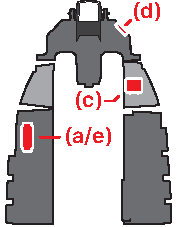
\includegraphics[width=\marginparwidth]{F16_proc_start-up_engine-start_v01.pdf}
        \caption{\textbf{Engine Start}}
    }
    \begin{subenumerate}
        \item \textbf{JFS Switch} \dotfill \textbf{START 2}
        \item \textbf{Throttle} \dotfill \textbf{IDLE} \\
        \hfill (once 20\% RPM reached)
        \item \textbf{SEC Light} \dotfill \textbf{OFF} 
        \item \textbf{ENGINE Warning Light} \dotfill \textbf{OFF} \\
        \hfill (once 60\% RPM reached)
        \item \textbf{JFS Switch} \dotfill \textbf{Confirm OFF}
    \end{subenumerate}\cbend}
    \blueitem{ENG Instruments}{
    \marginpar{
        \captionsetup{type=figure}
        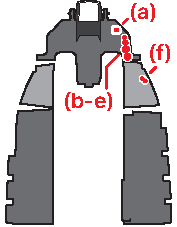
\includegraphics[width=\marginparwidth]{F16_proc_start-up_engine-instruments_v01.pdf}
        \caption{\textbf{ENG Instruments}}
    }
    \begin{subenumerate}
        \item \textbf{FUEL FLOW} --- 700-1700 PPH
        \item \textbf{OIL Pressure} --- 15 PSI (minimum)
        \item \textbf{NOZ POS} --- greater than 95\%
        \item \textbf{RPM} --- 62-80\% 
        \item \textbf{FTIT} --- 650C or less
        \item \textbf{HYD PRES A \& B} --- 2850-3250 PSI
    \end{subenumerate}}
\end{checklistenumerate}

\notebox{
    \begin{itemize}
        \item \textbf{Can close Canopy prior to advancing Throttle to IDLE to reduce cockpit noise}
    \end{itemize}
}

\clearpage

\subsection{POST-START}
\begin{checklistenumerate}
    \blueitem{TEST Panel}{
    \marginpar{
        \captionsetup{type=figure}
        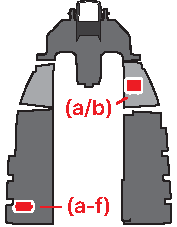
\includegraphics[width=\marginparwidth]{F16_proc_start-up_test-panel_v01.pdf}
        \caption{\textbf{TEST Panel}}
    }
    \begin{subenumerate}
        \item \textbf{PROBE HEAT Switch} \dotfill \textbf{PROBE HEAT} \\
        \hfill verify PROBE HEAT Caution Light --- off
        \item \textbf{PROBE HEAT Switch} \dotfill \textbf{TEST} \\
        \hfill verify PROBE HEAT Caution Light --- flashing
        \item \textbf{PROBE HEAT Switch} \dotfill \textbf{OFF}
        \item \textbf{FIRE \& OHEAT DETECT} \dotfill \textbf{TEST}
        \item \textbf{OXY QTY Test Switch} \dotfill \textbf{TEST}
        \item \textbf{MAL \& IND LTS Button} \dotfill \textbf{TEST}
    \end{subenumerate}}
    \blueitem{AVIONICS Panel}{\cbstart
    \marginpar{
        \captionsetup{type=figure}
        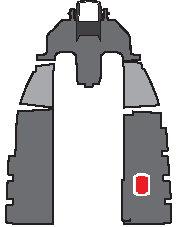
\includegraphics[width=\marginparwidth]{F16_proc_start-up_avionics-ins_v01.pdf}
        \caption{\textbf{Avionics \& INS}}
    }
    \begin{subenumerate}
        \item \textbf{MMC Switch} \dotfill \textbf{MMC}
        \item \textbf{ST STA Switch} \dotfill \textbf{ST STA}
        \item \textbf{MFD Switch} \dotfill \textbf{MFD}
        \item \textbf{UFC Switch} \dotfill \textbf{UFD}
        \item \textbf{GPS Switch} \dotfill \textbf{GPS}
        \item \textbf{DL Switch} \dotfill \textbf{DL}
        \item \textbf{MIDS LVT Knob} \dotfill \textbf{ON}
    \end{subenumerate}}
    \blueitem{INS Alignment}{
    \begin{subenumerate}
        \item \textbf{EGI/INS} \dotfill \textbf{Desired ALIGN Mode} \\
        \begin{itemize}
            \item \textbf{NORM} --- Full alignment, approx. 8 min
            \item \textbf{STOR HDG} --- Quick alignment, approx. 90 sec
        \end{itemize}
    \end{subenumerate}}
    \blueitem{SNSR PWR Panel}{
    \marginpar{
        \captionsetup{type=figure}
        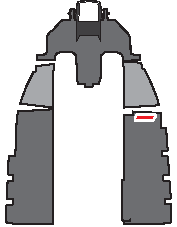
\includegraphics[width=\marginparwidth]{F16_proc_start-up_snsr-pwr_v01.pdf}
        \caption{\textbf{SNSR PWR Panel}}
    }
    \begin{subenumerate}
        \item \textbf{LEFT HDPT Switch} \dotfill \textbf{As Required} \\
        \hfill if HTS Pod installed
        \item \textbf{RIGHT HDPT Switch} \dotfill \textbf{As Required} \\
        \hfill if Targetting Pod installed
        \item \textbf{FCR Switch} \dotfill \textbf{FCR}
        \item \textbf{RDR ALT Switch} \dotfill \textbf{RDR ALT}
    \end{subenumerate}\cbend}
\end{checklistenumerate}

\clearpage

\begin{checklistenumerate}[resume]
    \blueitem{HUD Setup}{\cbstart
    \marginpar{
        \captionsetup{type=figure}
        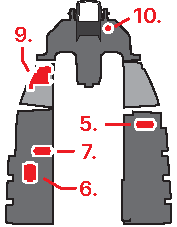
\includegraphics[width=\marginparwidth]{F16_proc_start-up_hud-sai_v01.pdf}
        \caption{\textbf{HUD, C\&I, ECM, SPD BRK, WHEELS Down, SAI}}
    }
    \begin{subenumerate}
        \item \textbf{HUD Control Panel} \dotfill \textbf{As Desired}
        \item \textbf{HUD Brightness} \dotfill \textbf{As Desired} 
    \end{subenumerate}\cbend}
    \blueitem{C\&I Knob}{\textbf{UFC}}
    \blueitem{ECM Panel}{\cbstart\textbf{As Desired}\cbend}
    \blueitem{SPD BRK Check}{\textbf{Cycle} (back to closed)}
    \blueitem{WHEELS Down Lights}{Verify \textbf{Three Green}}
    \blueitem{\cbstart  Standby Attitude Indicator\cbend}{\textbf{Set}}
    \blueitem{Tests \& Checks}{\hyperref[subsec:testschecks]{\textbf{See \Cref{subsec:testschecks} Tests \& Checks}}}
% \end{checklistenumerate}

% \clearpage

% \begin{checklistenumerate}[resume]
    \blueitem{Avionics Setup}{
    \marginpar{
        \captionsetup{type=figure}
        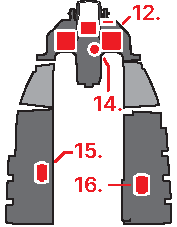
\includegraphics[width=\marginparwidth]{F16_proc_start-up_final-setup_v01.pdf}
        \caption{\textbf{Final Setup}}
    }
    \cbstart\textbf{Program As Required}}
    \blueitem{Canopy}{\textbf{Close and Lock}}
    \blueitem{Altimeter}{\textbf{Set and Check}}
    \blueitem{Exterior Lights}{\textbf{As Desired}}
    \blueitem{INS Knob}{\textbf{NAV}\cbend}
    \blueitem{NWS}{\textbf{Engage}}
    \blueitem{Throttle}{\textbf{Advance} (Check brakes \& NWS)}
    \blueitem{Flight Instruments}{\textbf{Check}}
\end{checklistenumerate}

% \clearpage

\warningbox{
    \begin{itemize}
        \item \textbf{Aircraft Rearming can interrupt INS align}
        \begin{itemize}
            \item If interrupted recycle INS knob to off, then back to align
            \item Recommend rearming either before or after INS align
        \end{itemize}
    \end{itemize}
}

\clearpage

\subsection{TESTS \& CHECKS}
\label{subsec:testschecks}
\begin{checklistenumerate}
    \blueitem{ENG SEC Mode}{
    \marginpar{
        \captionsetup{type=figure}
        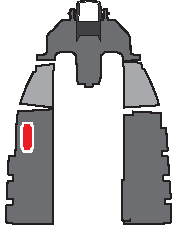
\includegraphics[width=\marginparwidth]{F16_proc_start-up_check-eng-sec_v01.pdf}
        \caption{\textbf{ENG SEC Mode}}
    }
    \begin{subenumerate}
        \item \textbf{ENG CONT Switch} \dotfill \textbf{SEC}
        \begin{itemize}
            \item \textbf{SEC Caution Light} --- \textbf{ON}
            \item \textbf{RPM} --- Stabilized
            \item \textbf{Throttle} --- Snap to \textbf{MIL}, then to \textbf{IDLE} when RPM reaches 85\% 
            \item \textbf{NOZ POS} --- < 10\% within 30s after \textbf{SEC} selection
        \end{itemize}
        \item \textbf{ENG CONT Switch} \dotfill \textbf{PRI}
        \begin{itemize}
            \item \textbf{SEC Caution Light} --- \textbf{OFF}
            \item \textbf{NOZ POS} --- > 94\% 
        \end{itemize}
    \end{subenumerate}}
    \blueitem{FLCS BIT}{
    \marginpar{
        \captionsetup{type=figure}
        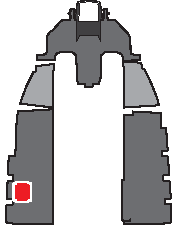
\includegraphics[width=\marginparwidth]{F16_proc_start-up_check-flcs-bit_v01.pdf}
        \caption{\textbf{FLCS BIT}}
    }
    \begin{subenumerate}
        \item \textbf{FLCS BIT Switch} \dotfill \textbf{BIT}
        \begin{itemize}
            \item \textbf{FLCP RUN Light} --- Illuminates
        \end{itemize}
        \item \textbf{BIT Completion}
        \begin{itemize}
            \item \textbf{Duration} --- Approx. 45s
            \item \textbf{FLCP RUN Light} --- Extinguishes
            \item \textbf{BIT Switch} --- Returns to \textbf{OFF}
            \item \textbf{FAIL Light} --- Verify \textbf{OFF}
            \item \textbf{FLCS Warning Light} --- Verify \textbf{OFF}
        \end{itemize}
    \end{subenumerate}}
\end{checklistenumerate}

\clearpage

\begin{checklistenumerate}[resume]
    \blueitem{FUEL QTY Check}{
    \marginpar{
        \captionsetup{type=figure}
        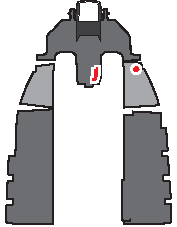
\includegraphics[width=\marginparwidth]{F16_proc_start-up_check-fuel-qty_v01.pdf}
        \caption{\textbf{FUEL QTY Check}}
    }
    \begin{subenumerate}
        \item \textbf{FUEL QTY SEL Knob} \dotfill \textbf{TEST}
        \begin{itemize}
            \item \textbf{FR/AL Pointers} --- 2000 $\pm$ 100 lbs
            \item \textbf{Totalizer} --- 6000 $\pm$ 100 lbs
        \end{itemize}
        \item \textbf{FUEL QTY SEL Knob} \dotfill \textbf{NORM}
        \begin{itemize}
            \item \textbf{AL Pointer} --- 2675/2810 lbs
            \item \textbf{FR POINTER} --- 3100/3250 lbs
        \end{itemize}
        \item \textbf{FUEL QTY SEL Knob} \dotfill \textbf{RSVR}
        \begin{itemize}
            \item Each indicator approx. 460/480 lbs
        \end{itemize}
        \item \textbf{FUEL QTY SEL Knob} \dotfill \textbf{INT WING}
        \begin{itemize}
            \item Each indicator approx. 525/550 lbs
        \end{itemize}
        \item \textbf{FUEL QTY SEL Knob} \dotfill \textbf{EXT WING}
        \begin{itemize}
            \item Each indicator approx. 2300/2420 lbs
            \hfill (if loaded)
        \end{itemize}
        \item \textbf{FUEL QTY SEL Knob} \dotfill \textbf{As Desired}
    \end{subenumerate}}
    \blueitem{DBU Check}{
    \marginpar{
        \captionsetup{type=figure}
        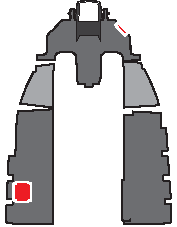
\includegraphics[width=\marginparwidth]{F16_proc_start-up_check-dbu_v01.pdf}
        \caption{\textbf{DBU Check}}
    }
    \begin{subenumerate}
        \item \textbf{DIGITAL BACKUP Switch} \dotfill \textbf{BACKUP}
        \begin{itemize}
            \item \textbf{DBU ON Light} --- \textbf{Illuminates}
        \end{itemize}
        \item Operate Controls --- check for normal control surface response
        \item \textbf{DIGITAL BACKUP Switch} \dotfill \textbf{OFF}
    \end{subenumerate}}
    \blueitem{Trim Check}{
    \marginpar{
        \captionsetup{type=figure}
        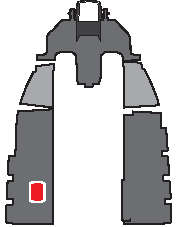
\includegraphics[width=\marginparwidth]{F16_proc_start-up_check-trim_v01.pdf}
        \caption{\textbf{Trim Check}}
    }
    \begin{subenumerate}
        \item \textbf{TRIM/AP DISC Swtich} \dotfill \textbf{DISC}
        \item \textbf{Stick Trim} \dotfill Activate in Pitch \& Roll
        \begin{itemize}
            \item No control surface motion 
            \item No TRIM wheel or indicator motion
        \end{itemize} 
        \item \textbf{TRIM/AP DISC Swtich} \dotfill \textbf{NORM}
        \item \textbf{Stick Trim} \dotfill Check \& Center
        \begin{itemize}
            \item Control surface motion 
            \item TRIM wheel motion
        \end{itemize} 
        \item \textbf{Yaw Trim Knob} \dotfill \textbf{Center}
    \end{subenumerate}}
\end{checklistenumerate}

\clearpage

\begin{checklistenumerate}[resume]
    \blueitem{MPO Check}{
    \marginpar{
        \captionsetup{type=figure}
        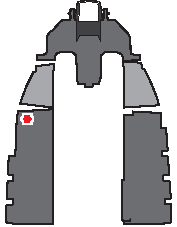
\includegraphics[width=\marginparwidth]{F16_proc_start-up_check-mpo_v01.pdf}
        \caption{\textbf{MPO Check}}
    }
    \begin{subenumerate}
        \item \textbf{Stick} \dotfill \textbf{Full Forward \& Hold}
        \item \textbf{MPO Switch} \dotfill \textbf{OVRD \& Hold}
        \begin{itemize}
            \item Horizontal Tail trailing edges move farther down
        \end{itemize} 
        \item \textbf{Stick \& MPO} \dotfill Release
    \end{subenumerate}}
    \blueitem{EPU Check}{
    \marginpar{
        \captionsetup{type=figure}
        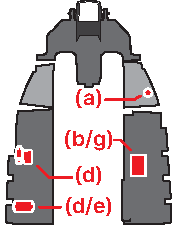
\includegraphics[width=\marginparwidth]{F16_proc_start-up_check-epu_v01.pdf}
        \caption{\textbf{EPU Check}}
    }
    \begin{subenumerate}
        \item \textbf{EPU FUEL Qty} \dotfill \textbf{95-102 Percent}
        \item \textbf{OXYGEN} \dotfill \textbf{100\%}
        \item \textbf{Throttle} \dotfill 10\% above \textbf{IDLE}
        \item \textbf{EPU/GEN TEST Switch} \dotfill \textbf{EPU/GEN \& Hold}
        \begin{itemize}
            \item \textbf{EPU AIR Light} --- \textbf{ON}
            \item \textbf{EPU GEN/PMG Lights} --- \textbf{OFF}
            \item \textbf{FLCS PWR Lights} --- \textbf{ON}
            \item \textbf{EPU Run Light} --- \textbf{ON} minimum 5s
        \end{itemize} 
        \item \textbf{EPU/GEN TEST Switch} \dotfill \textbf{OFF}
        \item \textbf{Throttle} \dotfill \textbf{IDLE}
        \item \textbf{OXYGEN} \dotfill \textbf{NORMAL}
    \end{subenumerate}}
\end{checklistenumerate}

\clearpage

\section{TAKEOFF \& LANDING}

\subsection{PRE-TAKEOFF}
\begin{checklistenumerate}
    \blueitem{ALT FLAPS Switch}{\textbf{Verify Norm}}
    \blueitem{Trim}{\textbf{Check}}
    \blueitem{ENG CONT Switch}{\textbf{Verify PRI}}
    \blueitem{Speedbrakes}{\textbf{Closed}}
    \blueitem{Canopy}{\textbf{Verify Closed \& Locked}}
    \blueitem{IFF}{\textbf{Set \& Check}}
    \blueitem{FUEL QTY Select Knob}{\textbf{NORM}}
    \blueitem{STORES CONFIG Switch}{\textbf{As Required}
    
    \begin{subitemize}
        \item \textbf{CAT I} --- \textbf{A-A Loadouts} 
        \item \textbf{CAT III} --- \textbf{A-G / Wing tank Loadouts}
    \end{subitemize}}
    \blueitem{PROBE HEAT Switch}{\textbf{PROBE HEAT}}
    \blueitem{Ejection Safety Lever}{\textbf{Arm (down)}}
    \blueitem{Flight Controls}{\textbf{Cycle}}
    \blueitem{Oil Pressure}{\textbf{15-65 psi}}
    \blueitem{TGP}{\textbf{STOW} (if installed)}
    \blueitem{Warning \& Caution Lights}{\textbf{Verify Off}}
\end{checklistenumerate}

\subsection{TAKEOFF}

\begin{checklistenumerate}
    \blueitem{Runup}{\cbstart
    \begin{subenumerate}
        \item \textbf{Brake} \dotfill \textbf{Hold}
        \item \textbf{Throttle} \dotfill \textbf{90\%}\cbend
    \end{subenumerate}}
    \blueitem{Runup Check}{
    \begin{subenumerate}
        \item \textbf{Parking Brake} \dotfill \textbf{Verify disengaged}
        \item \textbf{Engine Parameters} \dotfill \textbf{Nominal}
        \begin{itemize}
            \item \textbf{HYD/OIL PRES} --- \textbf{OFF}
            \item \textbf{Oil Pressure} --- \textbf{25-65psi}
            \item \textbf{FTIT} --- \textbf{less than 935deg}
            \item \textbf{HYD PRESS A \& B} --- \textbf{2850-3250psi}
        \end{itemize}
    \end{subenumerate}}
\end{checklistenumerate}

\clearpage

\begin{checklistenumerate}[resume]
    \blueitem{Takeoff Roll}{\cbstart
    \marginpar{
        \captionsetup{type=table}
        \centering
        \caption{\textbf{Takeoff Speeds}}
        \label{tab:proc:takeoff:speed}
        \begin{tabular}{c c}
            \toprule 
            \textbf{Weight} & \textbf{TO Speed} \\
            \textbf{[lbs]} & \textbf{[kts]} \\
            \midrule 
            20000 & 128 \\
            \midrule 
            24000 & 142 \\
            \midrule 
            28000 & 156 \\
            \midrule 
            32000 & 168 \\
            \midrule 
            36000 & 178 \\
            \midrule 
            40000 & 188 \\
            \midrule 
            44000 & 198 \\
            \bottomrule
        \end{tabular}
    }
    \begin{subenumerate}
        \item \textbf{Brake} \dotfill \textbf{Release}
        \item \textbf{Throttle} \dotfill \textbf{As Desired}\cbend
        \begin{itemize}
            \item \textbf{NOZ POS} --- \textbf{< 15\%} after 5 sec at \textbf{MIL/AB}
        \end{itemize}
    \end{subenumerate}
    
    At 70 kts

    \begin{subenumerate}[start=3]
        \item \textbf{NWS} \dotfill \textbf{Disengaged}
    \end{subenumerate}}
    \blueitem{Rotation}{\cbstart At 10-15kts below takeoff speed, reference \cref{tab:proc:takeoff:speed}

    \begin{subenumerate}
        \item \textbf{Attitude} \dotfill \textbf{8-12 deg nose high}
    \end{subenumerate}

    Once positive rate has been achieved
    
    \begin{subenumerate}[start=2]
        \item \textbf{Gear} \dotfill \textbf{UP}\cbend
    \end{subenumerate}}
\end{checklistenumerate}

\begin{figure}[htbp]
    \centering
    \begin{tikzpicture}[auto, node distance=10mm, x=1mm, y=1mm, very thick, line cap=round,
        >={Latex[round]}
        ]

        % coordinates
        \coordinate (startpoint) at (0,0);
        \coordinate (70kts) at (25,0);
        \coordinate (rotate) at (50,0);
        \coordinate (runwaystart) at (-5,-2.5);
        \coordinate (runwayend) at (70,-2.5);

        % runway
        \draw[thick, fill]
        ($(runwaystart)+(0,-0.25)$) -- ($(runwaystart)+(0,0.25)$) -- 
        ($(runwayend)+(0,0.25)$) -- ($(runwayend)+(0,-0.25)$) -- 
        cycle;

        % path
        \draw[ultra thick, ->]
        (startpoint) -- (70kts);
        \draw[ultra thick, ->]
        (70kts) -- (rotate);
        \draw[ultra thick, ->]
        (rotate) -- ++(5,0) arc (270:300:10) -- ++(30:10);

        % nodes
        \node[above, align=center] at (startpoint) {\small\textbf{Brakes} \\ \small\textbf{Runup}};
        \node[above, align=center] at (70kts) {\small\textbf{70kts} \\ \small\textbf{NWS Off}};
        \node[above, align=center] at (rotate) {\small\textbf{128-198kts} \\ \small\textbf{Rotate}};

    \end{tikzpicture}
    \caption{Takeoff Profile}
\end{figure}

\clearpage

\subsection{PRE-LANDING}

\begin{checklistenumerate}
    \blueitem{Fuel}{\textbf{Check}}
    \blueitem{Landing Light}{\textbf{ON}}
    \blueitem{Altimeter}{\textbf{Set \& Check}}
    \blueitem{Attitude References}{\textbf{Check}}
    \blueitem{Anti-Ice}{\textbf{As Required}}
    \blueitem{TGP}{\textbf{STOW} (if installed)}
\end{checklistenumerate}

\subsection{LANDING}

\begin{checklistenumerate}
    \blueitem{Approach}{Align aircraft with runway
    \marginpar{
        \captionsetup{type=figure}
        \centering
        \begin{tikzpicture}[auto, node distance=10mm, x=1mm, y=1mm, very thick, line cap=round,
            >={Latex[round]}
            ]

            % coordinates
            \coordinate (approach) at (5,-15);
            \coordinate (break) at (5,20);
            \coordinate (downwind) at (-15,20);
            \coordinate (base) at (-15,-15);
            \coordinate (final) at (-7.5,-22.5);
            \coordinate (shortfinal) at (0,-15);
            \coordinate (touchdown) at (0,0);
            \coordinate (rollout) at (0,20);

            % runway
            \draw[thick]
            ($(touchdown)+(-2,-5)$) -- ($(touchdown)+(2,-5)$) -- 
            ($(touchdown)+(2,25)$) -- ($(touchdown)+(-2,25)$) -- 
            cycle;
            \draw[thick]
            ($(touchdown)+(-1.33,-1)$) -- ($(touchdown)+(-1.33,1)$)
            ($(touchdown)+(-0.66,-1)$) -- ($(touchdown)+(-0.66,1)$)
            ($(touchdown)+(0.66,-1)$) -- ($(touchdown)+(0.66,1)$)
            ($(touchdown)+(1.33,-1)$) -- ($(touchdown)+(1.33,1)$);

            % pattern
            \draw[ultra thick, ->] 
            (approach) -- (break);
            \draw[ultra thick] 
            (break) arc (0:180:10);
            \draw[ultra thick, >->] 
            (downwind) -- (base);
            \draw[ultra thick] 
            (base) arc (180:270:7.5);
            \draw[ultra thick] 
            (final) arc (270:360:7.5);
            \draw[ultra thick, >-] 
            (shortfinal) -- (touchdown);
            \draw[ultra thick, ->] 
            (touchdown) -- (rollout);

            % nodes
            \node[right] at (approach) {\textbf{1.}};
            \node[right] at (break) {\textbf{2.}};
            \node[left] at (downwind) {\textbf{3.}};
            \node[left] at (base) {\textbf{4.}};
            \node[below] at (final) {\textbf{5.}};
            \node[left] at (shortfinal) {\textbf{6.}};
            \node[left=2mm] at (touchdown) {\textbf{7.}};
            \node[left=2mm] at (rollout) {\textbf{8.}};

        \end{tikzpicture}
        \caption{Overhead Pattern}
        \label{fig:proc:landing:overhead}
    }

    \begin{subitemize}
        \item \textbf{Altitude} --- \textbf{1500 ft AGL}
        \item \textbf{Airspeed} --- \textbf{300 kts CAS}
    \end{subitemize}}
    \blueitem{Overhead Break}{Break left/right over desired touchdown point, maintain \underline{level turn}

    \begin{subitemize}
        \item \textbf{Speedbrakes} --- \textbf{As Required}
        \item \textbf{Throttle} --- \textbf{As Required}
        \item \textbf{Bank} --- \textbf{70 deg}
        \item \textbf{Break} --- \textbf{3-4 G}
    \end{subitemize}}
    \blueitem{Downwind Leg}{Roll out on opposite heading of runway, trim for 11 deg AoA

    \begin{subitemize}
        \item \textbf{Altitude} --- \textbf{1500 ft AGL}
        \item \textbf{Airspeed} --- \textbf{200-220 kts CAS}
        \item \textbf{Gear} --- \textbf{Down}
    \end{subitemize}}
    \blueitem{Base Turn}{Initiate abeam of desired touchdown point (wingtip at end of runway)

    \begin{subitemize}
        \item \textbf{Attitude} --- \textbf{8-10 deg nose low}
        \item \textbf{AoA} --- \textbf{11 deg}
    \end{subitemize}}
    \blueitem{Final Turn}{Use throttle to maintain AoA, stick to maintain attitude, goal is to roll wings-level at

    \begin{subitemize}
        \item \textbf{1 mile} from desired touchdown point
        \item \textbf{Altitude} --- \textbf{300 ft AGL}
        % \item \textbf{AoA} --- \textbf{11 deg}
        \item \textbf{Flightpath} --- align  with \textbf{2.5 deg HUD marker} and runway threshold
    \end{subitemize}}
\end{checklistenumerate}

\clearpage

\begin{checklistenumerate}[resume]
    \blueitem{Short Final}{Once over runway
    
    \marginpar{
        \captionsetup{type=figure}
        \centering
        \begin{tikzpicture}[auto, node distance=10mm, x=1mm, y=1mm, very thick, line cap=round,
            >={Latex[round]}
            ]

            % coordinates
            \coordinate (approach) at (5,-15);
            \coordinate (break) at (5,20);
            \coordinate (downwind) at (-15,20);
            \coordinate (base) at (-15,-15);
            \coordinate (final) at (-7.5,-22.5);
            \coordinate (shortfinal) at (0,-15);
            \coordinate (touchdown) at (0,0);
            \coordinate (rollout) at (0,20);

            % runway
            \draw[thick]
            ($(touchdown)+(-2,-5)$) -- ($(touchdown)+(2,-5)$) -- 
            ($(touchdown)+(2,25)$) -- ($(touchdown)+(-2,25)$) -- 
            cycle;
            \draw[thick]
            ($(touchdown)+(-1.33,-1)$) -- ($(touchdown)+(-1.33,1)$)
            ($(touchdown)+(-0.66,-1)$) -- ($(touchdown)+(-0.66,1)$)
            ($(touchdown)+(0.66,-1)$) -- ($(touchdown)+(0.66,1)$)
            ($(touchdown)+(1.33,-1)$) -- ($(touchdown)+(1.33,1)$);

            % pattern
            \draw[ultra thick, ->] 
            (approach) -- (break);
            \draw[ultra thick] 
            (break) arc (0:180:10);
            \draw[ultra thick, >->] 
            (downwind) -- (base);
            \draw[ultra thick] 
            (base) arc (180:270:7.5);
            \draw[ultra thick] 
            (final) arc (270:360:7.5);
            \draw[ultra thick, >-] 
            (shortfinal) -- (touchdown);
            \draw[ultra thick, ->] 
            (touchdown) -- (rollout);

            % nodes
            \node[right] at (approach) {\textbf{1.}};
            \node[right] at (break) {\textbf{2.}};
            \node[left] at (downwind) {\textbf{3.}};
            \node[left] at (base) {\textbf{4.}};
            \node[below] at (final) {\textbf{5.}};
            \node[left] at (shortfinal) {\textbf{6.}};
            \node[left=2mm] at (touchdown) {\textbf{7.}};
            \node[left=2mm] at (rollout) {\textbf{8.}};

        \end{tikzpicture}
        \caption{Overhead Pattern}
    }

    \begin{subitemize}
        \item \textbf{Flightpath} --- shift \textbf{300-500 ft} down runway
        \item \textbf{Flare} --- gently pull back on stick
        \item \textbf{Throttle} --- \textbf{Idle}
        \item \textbf{AoA} --- \textbf{< 13 deg}
    \end{subitemize}}
    \blueitem{Touchdown}{}
    \blueitem{Roll-Out}{Maintain nose-high position for \underline{aerobraking} until 100 kts
    \begin{subitemize}
        \item \textbf{AoA} --- \textbf{< 13 deg}
        \item \textbf{Speedbrakes} --- \textbf{Open}
        \item \textbf{Brakes} --- \textbf{As Required}
    \end{subitemize}}
    \blueitem{Taxi}{
    \begin{subitemize}
        \item \textbf{NWS} --- \textbf{Engaged}
    \end{subitemize}}
\end{checklistenumerate}

\notebox{
    \textbf{\Cref{fig:proc:landing:overhead} is illustrated with extended approach and downwind sections for clarity}
}

\clearpage

\subsection{POST-LANDING}
\begin{checklistenumerate}
    \blueitem{PROBE HEAT Switch}{\textbf{OFF}}
    \blueitem{ECM Power}{\textbf{OFF}}
    \blueitem{Speedbrakes}{\textbf{Close}}
    \blueitem{Ejection Safety Lever}{\textbf{Safe (up)}}
    \blueitem{IFF Master Knob}{\textbf{STBY}}
    \blueitem{Landing/Taxi Light}{\textbf{As Desired}}
    \blueitem{Armament Switches}{\textbf{Safe}}
    \blueitem{Avionics}{\textbf{Off}
    \begin{subitemize}
        \item \textbf{HUD Thumbwheels} \dotfill \textbf{Off}
        \item \textbf{SNSR PWR Switches} \dotfill \textbf{Off}
        \item \textbf{AVIONICS PWR Switches} \dotfill \textbf{Off}
    \end{subitemize}}
    \blueitem{Engine Shutdown}{
    \begin{subenumerate}
        \item \textbf{Throttle} \dotfill \textbf{Off}
        \item \textbf{Lights} \dotfill \textbf{Check}
        \begin{itemize}
            \item \textbf{JFS Light} --- \textbf{Off}
            \item \textbf{EPU GEN Light} --- \textbf{Off}
            \item \textbf{EPU PMG Light} --- \textbf{Off}
        \end{itemize}
        \item \textbf{Main PWR Switch} \dotfill \textbf{OFF}
    \end{subenumerate}}
    \blueitem{Oxygen Regulator}{\textbf{Off}}
    \blueitem{Canopy}{\textbf{Open}}
\end{checklistenumerate}

\clearpage

\section{IN-FLIGHT}

\subsection{AIR-TO-AIR REFUELING}

\begin{checklistenumerate}
    \blueitem{Safe Aircraft}{
    \marginpar{
        \captionsetup{type=figure}
        \fbox{
            \begin{minipage}[t][50mm][t]{\marginparwidth}
                \center{\textbf{Refueling Areas}}
                \begin{itemize}[leftmargin=1em]
                    \item stretch-goal figure
                    \item show top-down view of tanker
                    \item label areas
                    \begin{itemize}
                        \item observation area
                        \item refueling area
                        \item reform area
                    \end{itemize}
                \end{itemize}
            \end{minipage}
        }
        \caption{Refueling Areas}
    }
    \begin{subenumerate}
        \item \textbf{Master Arm} \dotfill \textbf{OFF}
        \item \textbf{Laser Arm} \dotfill \textbf{OFF}
        \item \textbf{RF Switch} \dotfill \textbf{SILENT}
    \end{subenumerate}}
    \blueitem{Configure for Refueling}{
    \begin{subenumerate}
        \item \textbf{AIR REFUEL Switch}\cbstart \dotfill \textbf{Open}
        \item \textbf{AR Status Light} \dotfill \textbf{Verify RDY}\cbend
        \item \textbf{HOT MIC/CIPHER Switch} \dotfill \textbf{HOT MIC}
        \item \textbf{Exterior Lights} \dotfill \textbf{As required}
        \item \textbf{DED BINGO Page} \dotfill \textbf{Monitor}
    \end{subenumerate}
    
    If DED mirroring to HUD is desired 
    
    \begin{subenumerate}[start=6]
        \item \textbf{DED Data/PFL Switch} \dotfill \textbf{DED Data} 
    \end{subenumerate}}
    \blueitem{Refuel\cbstart}{
    \marginpar{
        \captionsetup{type=figure}
        \fbox{
            \begin{minipage}[t][50mm][t]{\marginparwidth}
                \center{\textbf{Director Lights}}
                \begin{itemize}[leftmargin=1em]
                    \item stretch-goal figure
                    \item show tanker director lights
                    \item show ``flat'' rather than in perspective
                    \item include centerline stripe
                \end{itemize}
            \end{minipage}
        }
        \caption{Tanker Director Lights}
    }
    \begin{subitemize}
        \item Fly into refueling area and allow boom operator to fly boom into refueling port
        \item \textbf{AR/NWS Light} illuminates to indicate contact
        \item Reference director lights to maintain position within boom limits
        \item Monitor refueling progress on DED/HUD
    \end{subitemize}}
    \blueitem{Post-Refueling}{
    \begin{subenumerate}
        \item \textbf{A/R DISC Button} \dotfill \textbf{Press}
        \item \textbf{AIR REFUEL Switch} \dotfill \textbf{Close}\cbend
        \item \textbf{HOT MIC/CIPHER Switch} \dotfill \textbf{OFF}
        \item \textbf{FUEL QTY} \dotfill \textbf{Check}
        \item \textbf{AR Status Light} \dotfill \textbf{Verify Off}
        \item \textbf{Exterior Lights} \dotfill \textbf{As required}
    \end{subenumerate}}
    \blueitem{Rearm Aircraft}{
    \begin{subenumerate}
        \item \textbf{RF Switch} \dotfill \textbf{As Required}
        \item \textbf{Laser Arm} \dotfill \textbf{As Required}
        \item \textbf{Master Arm} \dotfill \textbf{As Required}
    \end{subenumerate}}
\end{checklistenumerate}

\marginfigrestore

\cleardoublepage